\documentclass[11pt]{article}

\usepackage[margin=1in]{geometry}
\usepackage{amsmath,amssymb}
\usepackage{booktabs}
\usepackage{graphicx}
\usepackage{microtype}
\usepackage{hyperref}
\usepackage{url}
\usepackage{enumitem}
\usepackage{caption}

\hypersetup{colorlinks=true,linkcolor=black,citecolor=black,urlcolor=blue,pdftitle={Fikra Benchmark Phase 1: Comparative Evaluation of Four LLM Configurations Across Reasoning, Instruction Following, Mathematics, and Tool Use},pdfauthor={James Miano}}
\graphicspath{{figures/}}

\title{Fikra Benchmark Phase 1: Comparative Evaluation of Four LLM Configurations Across Reasoning, Instruction Following, Mathematics, and Tool Use}
\author{James Miano\\Lacesse Ventures (operator of the Fikra API)}
\date{September 2026}

\begin{document}
\maketitle

\begin{abstract}
This paper reports Phase 1 of an author-conducted evaluation of four language-model configurations served through the Fikra API; the author operates the Fikra API (see Disclosure). The evaluation uses a frozen 500-task suite assembled from MMLU-Pro, GPQA-Diamond, GSM8K, IFEval, LiveCodeBench, BFCL, and a Fikra-owned FRES set. Four configurations were evaluated under a common generation protocol, producing 2,000 planned model--task evaluations. Of these, 1,894 completed successfully (94.7\%), with 395 of the 500 frozen tasks (including tasks from the two unscored components) having successful results for all four configurations. The final scored analysis covers GPQA-Diamond, GSM8K, MMLU-Pro, IFEval, and BFCL; LiveCodeBench and FRES are explicitly excluded because reliable evaluation environments were not established. The completed results show heterogeneous capability profiles rather than a single uniform ordering across task families. Observed scores range from 46--88\% on GPQA-Diamond, 84--94.67\% on GSM8K, 29.03--37\% on MMLU-Pro, 68--86.67\% on strict IFEval, and 54--86\% on BFCL. Execution measurements also vary substantially, including median total latency from 1.60 s to 16.07 s across the four configurations. The study documents both capability results and practical evaluation limitations, including incomplete coverage and evaluator compatibility issues. The resulting artifact package provides the experiment manifest, benchmark artifact, raw results, diagnostics, and analysis records needed to reproduce or extend the study.
\end{abstract}

\section{Introduction}
Selecting a language model for a deployed system is not equivalent to selecting the model with the highest score on one benchmark. Different evaluations probe different properties: broad knowledge and reasoning, mathematical problem solving, instruction following, and structured tool invocation. In addition, deployed systems expose operational properties such as response latency and failure behavior. A useful empirical evaluation therefore needs to preserve the distinction between capability dimensions rather than collapsing heterogeneous measurements into an unsupported universal ranking.

This paper reports an author-conducted evaluation of four LLM configurations served through the Fikra API. The author operates the Fikra API, and the FRES set is Fikra-owned (see Disclosure). The objective is descriptive: characterize the observed behavior of the configurations under a fixed evaluation protocol and document the conditions under which those measurements were obtained. The study is not intended to establish a universal best model, nor does it claim that the observed ordering generalizes to all providers, endpoints, prompts, or workloads.

The evaluation suite contains 500 frozen tasks drawn from seven sources. MMLU-Pro provides a broad, reasoning-focused multiple-choice evaluation \cite{wang2024mmlupro}; GPQA targets difficult graduate-level scientific questions \cite{rein2023gpqa}; GSM8K evaluates grade-school mathematical reasoning \cite{cobbe2021gsm8k}; IFEval tests verifiable instruction following \cite{zhou2023ifeval}; LiveCodeBench was selected as the coding component \cite{jain2024livecodebench}; and BFCL evaluates function calling using structured validation including AST-based checking \cite{patil2025bfcl}. A seventh component, FRES, is a Fikra-owned evaluation set.

The primary research questions are:
\begin{enumerate}[leftmargin=*]
    \item How do the four configurations differ across heterogeneous capability categories?
    \item How complete and comparable are the resulting measurements when model--task execution failures are treated separately from incorrect answers?
    \item What execution characteristics accompany the observed capability measurements?
    \item What methodological limitations arise when public evaluators are reproduced in an API-based experimental environment?
\end{enumerate}

The principal contributions are a documented frozen evaluation suite, a reproducible four-configuration evaluation record, a capability-and-execution analysis, and an explicit accounting of incomplete and excluded evaluations. The work also provides an empirical basis for subsequent research into task-aware model routing without evaluating a router in this paper.

\section{Evaluation Landscape}
The benchmark combines evaluation families with different semantics. MMLU-Pro was designed as a more challenging and reasoning-focused successor to MMLU, using ten answer choices and filtering questions intended to improve discriminative power \cite{wang2024mmlupro}. GPQA consists of graduate-level questions written by domain experts in biology, physics, and chemistry and is intended to resist straightforward web search \cite{rein2023gpqa}. GSM8K contains linguistically diverse grade-school mathematics problems requiring multi-step calculation \cite{cobbe2021gsm8k}.

IFEval evaluates verifiable instructions such as required phrases, formatting constraints, and length constraints. Its original design emphasizes deterministic automatic verification rather than subjective judging \cite{zhou2023ifeval}. BFCL focuses on function calling and supports serial and parallel calls, with AST-based validation designed to make structured comparison scalable \cite{patil2025bfcl}. LiveCodeBench was included in the frozen design because it evaluates contemporary coding tasks while emphasizing temporal freshness and contamination resistance \cite{jain2024livecodebench}. It was not, however, scored in the final analysis because the required execution environment could not be established reliably.

The combination is intentionally heterogeneous. A result on one component is not treated as a proxy for another component. In particular, function-calling performance is reported separately from conventional reasoning and mathematics, and instruction following is reported separately from both.

\section{Benchmark Design}
\subsection{Frozen task composition}
The benchmark contains 500 tasks:

\begin{table}[t]
\centering
\caption{Frozen benchmark composition.}
\label{tab:composition}
\begin{tabular}{lr}
\toprule
Dataset & Tasks \\
\midrule
MMLU-Pro & 100 \\
GPQA-Diamond & 50 \\
GSM8K & 75 \\
IFEval & 75 \\
LiveCodeBench & 100 \\
BFCL & 50 \\
FRES & 50 \\
\midrule
Total & 500 \\
\bottomrule
\end{tabular}
\end{table}

The benchmark was frozen on 26 September 2026. The resulting benchmark SHA-256 is \texttt{bf904af6e4a7f909c92642f2299f1001c7f1aff88894684fd61f2e799df72bfb}. Dataset revisions were recorded in the experiment artifacts. Restricted source material, including gated benchmark question text where applicable, is not reproduced in the public manuscript source.

\subsection{Model configurations}
The evaluated configurations are listed below. Configuration names are Fikra product labels and do not denote upstream parameter counts. The two GPT-OSS-based configurations use the open-weight models of \cite{openai2025gptoss}. The configurations are evaluated as exposed by the API, including any serving-layer processing.
\begin{table}[t]
\centering
\caption{Evaluated Fikra configurations and upstream models.}
\label{tab:models}
\begin{tabular}{ll}
\toprule
Configuration & Upstream model \\
\midrule
Fikra Flash & GPT-OSS 20B \\
Fikra Pro 20B & Qwen 3.8 27B \\
Fikra Pro 120B & GPT-OSS 120B \\
Fikra Qwen Max & Qwen 3.8 Max \\
\bottomrule
\end{tabular}
\end{table}

The evaluation unit is one model configuration paired with one frozen task. Four configurations applied to 500 tasks yield 2,000 planned evaluations.

\subsection{Generation protocol}
Unless an evaluator required otherwise, requests used temperature 0, top-$p$ 1, one attempt per model--task pair, and a maximum output length of 4,096 tokens. The same frozen task wording was used across configurations. No external retrieval or human intervention was used during generation. The raw record stores task identifiers, model identifiers, response data, timing fields, token usage where available, HTTP/API status, and failure information.

\section{Evaluation Methodology}
\subsection{Completeness}
A successful generation and a correct answer are separate concepts. Failed or missing model--task executions are therefore not counted as incorrect answers. The run completed 1,894 of 2,000 planned evaluations, corresponding to 94.7\% successful execution coverage. Fikra Flash completed 499 tasks, Fikra Pro 20B completed 395, Fikra Pro 120B completed 500, and Fikra Qwen Max completed 500. A total of 395 benchmark tasks have successful results for all four configurations. These counts span all 500 frozen tasks, including the 150 LiveCodeBench and FRES tasks that are not scored; they describe generation coverage, not coverage of the scored analysis.

\begin{table}[t]
\centering
\caption{Evaluation coverage for the four model configurations.}
\label{tab:coverage}
\begin{tabular}{lrrr}
\toprule
Model & Successful & Planned & Coverage \\
\midrule
Fikra Flash & 499 & 500 & 99.8\% \\
Fikra Pro 20B & 395 & 500 & 79.0\% \\
Fikra Pro 120B & 500 & 500 & 100.0\% \\
Fikra Qwen Max & 500 & 500 & 100.0\% \\
\midrule
Total & 1,894 & 2,000 & 94.7\% \\
\bottomrule
\end{tabular}
\end{table}


The incomplete coverage is concentrated in Fikra Pro 20B and a single Fikra Flash evaluation. MMLU-Pro is particularly important because the Pro 20B result contains only 31 successful evaluations, of which 9 were correct. That result is reported descriptively but is not treated as equivalent to a complete 100-task measurement.

\subsection{Scoring}
The study uses deterministic or benchmark-native scoring wherever available. GPQA-Diamond uses exact answer-choice matching; GSM8K uses normalized final-answer matching; MMLU-Pro uses answer-choice matching; IFEval uses its verification logic; and BFCL uses the official AST-checking logic in standalone form.

Two evaluator qualifications are material. First, the IFEval implementation required compatibility-oriented keyword-argument sanitization because 116 instruction entries contained task keyword arguments that were not accepted by individual evaluator signatures. The underlying verification logic was retained, but the installation should not be described as an untouched upstream evaluator. Second, the complete BFCL evaluator stack encountered dependency/API compatibility problems. Final BFCL scoring therefore used the official BFCL AST-checking logic standalone, bypassing provider-handler and tree-sitter components that prevented the complete stack from executing.

\subsection{Excluded components}
LiveCodeBench and FRES were intentionally excluded from the final scored analysis because reliable evaluation environments could not be established under the frozen experiment. No score is estimated, imputed, or inferred for either component. The frozen benchmark definition retains them as part of the original 500-task design, while the reported capability analysis explicitly excludes them.

\section{Results}
\subsection{Capability results}
Table~\ref{tab:results} reports the completed scored components. The table is intentionally dataset-native: no aggregate score is designated as authoritative because the components have different evaluation semantics and coverage is incomplete.

\begin{table}[t]
\centering
\caption{Observed scores on the completed scored benchmark components. Percentages are calculated over successful evaluations for the corresponding model and dataset. Pro 20B's MMLU-Pro result is based on 21/31 successful evaluations and is therefore not comparable to a complete 100-task run.}
\label{tab:results}
\begin{tabular}{lrrrr}
\toprule
Dataset & Flash & Pro 20B & Pro 120B & Qwen Max \\
\midrule
GPQA-Diamond & 48.00 & 46.00 & 66.00 & 88.00 \\
GSM8K & 85.33 & 84.00 & 84.00 & 94.67 \\
MMLU-Pro & 77.00 & 67.74$^{\dagger}$ & 82.00 & 90.00 \\
IFEval (strict) & 68.00 & 76.00 & 72.00 & 86.67 \\
IFEval (loose) & 69.33 & 78.67 & 76.00 & 88.00 \\
BFCL & 54.00 & 86.00 & 58.00 & 82.00 \\
\bottomrule
\end{tabular}
\\[-2pt]
{\footnotesize $^{\dagger}$ 21/31 successful Pro 20B evaluations. LiveCodeBench and FRES were excluded from final scored analysis.}
\end{table}


\begin{figure}[t]
\centering
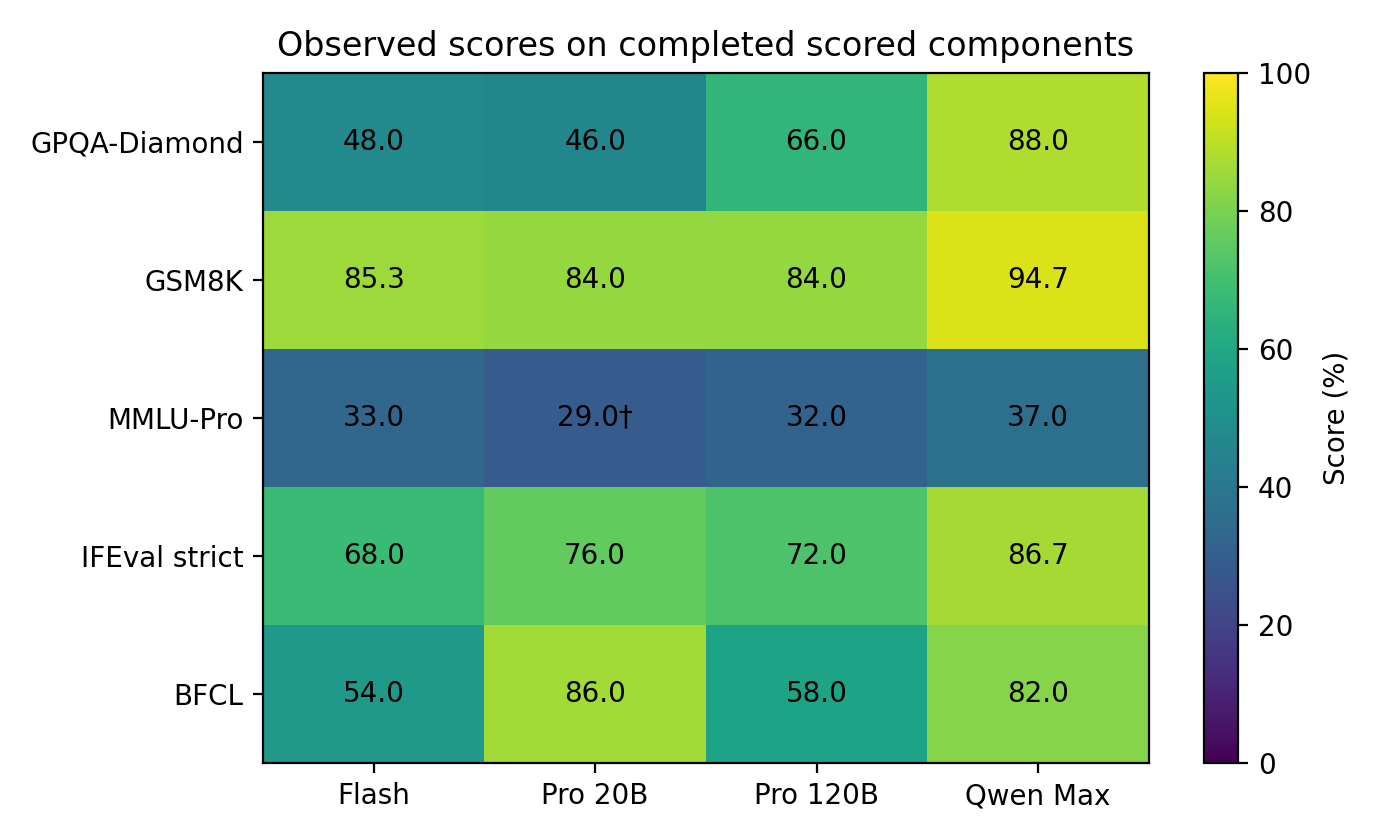
\includegraphics[width=0.96\linewidth]{capability_matrix.png}
\caption{Observed scores for the completed scored components. The Pro 20B MMLU-Pro value is based on incomplete coverage.}
\label{fig:matrix}
\end{figure}

On GPQA-Diamond, observed scores range from 46.00\% for Pro 20B to 88.00\% for Qwen Max. On GSM8K, all configurations perform relatively strongly, with scores from 84.00\% to 94.67\%. MMLU-Pro scores are lower, ranging from 29.03\% to 37.00\%, although the Pro 20B result is based on only 31 successful evaluations. Strict IFEval scores range from 68.00\% to 86.67\%, while BFCL scores range from 54.00\% to 86.00\%.

These measurements demonstrate that capability profiles vary by evaluation family. The same configuration can occupy materially different positions across reasoning, mathematics, instruction following, and function calling. Consequently, the completed results do not support a single universal ordering across all measured capabilities.

Sample sizes are small. At $n=50$, $n=75$, and $n=100$, a 95\% Wilson interval around an observed accuracy extends up to roughly $\pm$13, $\pm$11, and $\pm$10 percentage points respectively, so small differences between configurations, particularly on GPQA-Diamond, BFCL, and MMLU-Pro, should not be read as reliable orderings. In addition, percentages are computed over each configuration's successful evaluations, so Pro 20B is scored on a different and possibly easier subset of tasks than the other configurations; comparisons involving Pro 20B, including its latency, should be read with that in mind. A common-task comparison is left to future work.

\subsection{Function calling}
The BFCL aggregate results conceal substantial category variation. The four evaluated categories were simple Python, multiple calls, parallel calls, and parallel multiple calls. All four configurations achieved 90\% or higher on simple Python except Flash at 85\%, and all achieved 100\% on the multiple-call category. The largest differences occur in parallel categories: Flash scored 0/10 on both parallel categories; Pro 20B scored 6/10 and 9/10; Pro 120B scored 0/10 and 1/10; and Qwen Max scored 7/10 and 6/10.

This is a concrete reason to report tool-use behavior separately from conventional reasoning scores. The BFCL measurements are not interchangeable with GPQA, GSM8K, or MMLU-Pro measurements.

\subsection{Instruction following}
Strict IFEval scores were 68.00\% for Flash, 76.00\% for Pro 20B, 72.00\% for Pro 120B, and 86.67\% for Qwen Max. Loose scores were 69.33\%, 78.67\%, 76.00\%, and 88.00\%, respectively. The strict and loose results are both retained because they represent distinct evaluation outputs from the benchmark's verification logic.

\section{Operational Performance}
Capability measurements were accompanied by execution measurements. Table~\ref{tab:latency} reports medians from successful calls. These values describe the observed API execution conditions of this experiment rather than intrinsic, provider-independent model latency. The values of $n$ in Table~\ref{tab:latency} count calls with recorded timing fields and may be smaller than the completed counts in Table~\ref{tab:coverage}. Requests were issued concurrently (12 workers, approximately 80 requests per minute), so latency and time to first token may include queueing, retry, and rate-limit effects in addition to model inference time.

\begin{table}[t]
\centering
\caption{Median execution measurements from successful calls. These measurements describe the observed Fikra API execution conditions of this experiment and are not provider-independent intrinsic model latencies.}
\label{tab:latency}
\begin{tabular}{lrrrr}
\toprule
Model & $n$ & TTFT (ms) & Latency (ms) & Output tokens \\
\midrule
Fikra Flash & 444 & 1967.4 & 3419.6 & 366.5 \\
Fikra Pro 20B & 247 & 880.7 & 1602.2 & 139.0 \\
Fikra Pro 120B & 452 & 2010.7 & 3297.9 & 410.0 \\
Fikra Qwen Max & 500 & 13289.5 & 16065.4 & 529.5 \\
\bottomrule
\end{tabular}
\end{table}


The observed median total latency ranged from 1.60 s for Pro 20B to 16.07 s for Qwen Max. Median time to first token ranged from 0.88 s to 13.29 s. Output length also differed materially. These measurements illustrate why a deployment evaluation can require both capability and execution dimensions.

\begin{figure}[t]
\centering
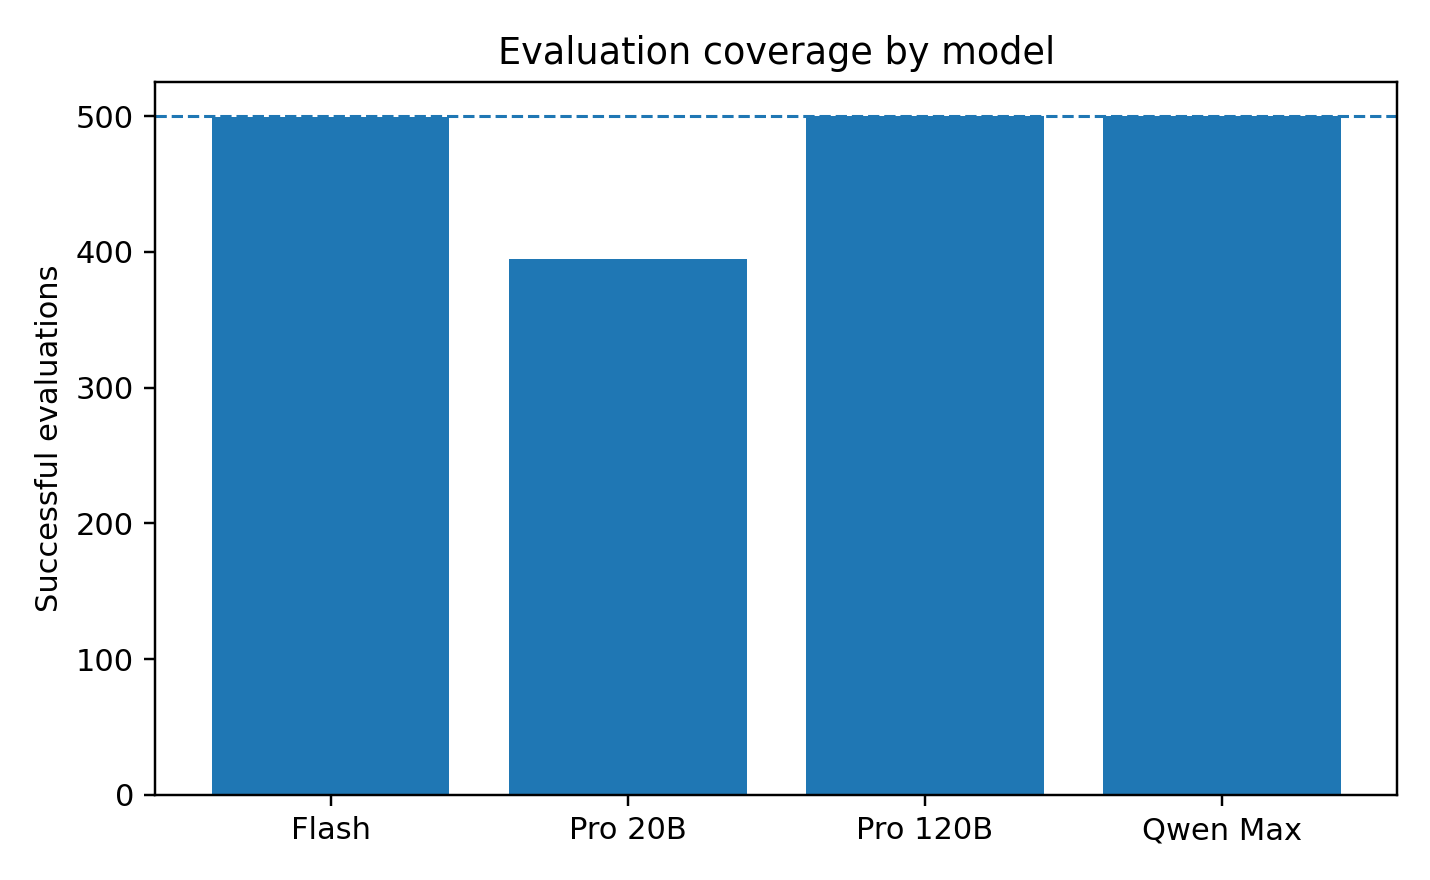
\includegraphics[width=0.88\linewidth]{coverage.png}
\caption{Successful model--task evaluations by configuration. The dashed line represents the 500-task target.}
\label{fig:coverage}
\end{figure}

\section{Methodological Findings}
The experiment exposed practical differences between reproducing a benchmark definition and reproducing its full evaluator environment. The frozen task set can be preserved and hashed, while the evaluator may still depend on package versions, provider interfaces, runtime assumptions, or generated response schemas.

The IFEval compatibility issue demonstrates that a public evaluator may require small interface adaptations even when the underlying verification rules are retained. The BFCL experience demonstrates a stronger form of environment dependence: the complete evaluation stack could not be executed under the available dependency/API environment, while the benchmark's official AST-checking logic could still be applied independently to suitable model outputs.

The experiment also shows why evaluation coverage should be published alongside accuracy. A missing response is an execution observation, not evidence that a model produced an incorrect answer. Treating the two as identical would confound infrastructure reliability with model capability.

\section{Discussion}
The completed results support three bounded observations. First, the four configurations have differentiated capability profiles across the measured task families. Second, tool-use performance can differ substantially from conventional reasoning and mathematics performance, making a single capability dimension insufficient for deployment-oriented evaluation. Third, execution characteristics such as latency and successful-call coverage are relevant empirical dimensions alongside benchmark accuracy.

The results do not establish a universal best configuration. They also do not establish that model size, upstream model family, or any other single model attribute causally explains the observed differences. The experiment measures configurations as exposed through the Fikra API under the stated protocol; provider-side implementation, serving infrastructure, prompt handling, and runtime conditions can contribute to the observations.

The heterogeneous profiles motivate subsequent research into task-aware routing. A routing system could use task characteristics and operational constraints to select among configurations, but that hypothesis requires a separate evaluation. No claim about the quality, cost, or latency of any routing system is made in this paper.

\section{Limitations}
The primary limitation is incomplete evaluation coverage. Although 1,894 of 2,000 planned evaluations succeeded, 106 did not, and Pro 20B has materially lower coverage than the other configurations. The MMLU-Pro Pro 20B result is consequently not equivalent to a complete 100-task result.

A second limitation is evaluator compatibility. IFEval required compatibility-oriented argument sanitization, and BFCL required standalone use of its official AST-checking logic rather than execution of the complete evaluator stack. These decisions are documented to make the result interpretable and reproducible, but they remain methodological qualifications.

A third limitation is the exclusion of LiveCodeBench and FRES from final scoring. No scores are reported for either component. Independent reproduction of those evaluations in a reliable environment would extend the study but would constitute additional experimental work rather than a value that can be inferred from the existing record.

A further limitation concerns harness validity. Several absolute scores are lower than values commonly reported for the underlying open-weight models, notably on MMLU-Pro, and both GPT-OSS-based configurations scored near zero on the parallel BFCL categories. Possible contributors include the 4,096-token output cap truncating long reasoning before a final answer, answer-extraction or output-format handling, differing reasoning-effort behavior across configurations, and the temperature-0 setting. These possibilities were not isolated in Phase 1, so the scores should be read as measurements of these configurations under this specific harness, not as estimates of the upstream models' peak capability. Manual verification of a sample of responses is a priority for the next phase.

Finally, the study does not define an authoritative aggregate score. Such a score would require explicit decisions about weighting heterogeneous capabilities and handling incomplete coverage. The paper therefore reports dataset-native measurements and common-coverage facts rather than manufacturing a universal ranking.

\section{Reproducibility and Research Artifacts}
The research package contains the frozen benchmark artifact, experiment manifest, raw result files, notebook used for the production run, dataset revision metadata, evaluator diagnostics, scoring record, research claims, and reproducibility notes. The benchmark hash is recorded above and the run is identified as \texttt{fikra-benchmark-phase1-2026-09-26-4model}; the experiment identifier is \texttt{fikra-phase1-2026-09-26-v1}.

Restricted benchmark content and credentials are not included in the manuscript source or the public repository. The public paper source is deliberately smaller than the complete research archive because posted manuscript source files are themselves publicly downloadable. This separation keeps the manuscript focused on the files required to compile the paper; the larger evidence archive is provided in the repository.

Code, benchmark metadata, and raw results are publicly available at \url{https://github.com/Fikra-API/fikra-benchmark} and archived on Zenodo (\url{https://doi.org/10.5281/zenodo.23047091}). The study was conducted by the author, who operates the Fikra API. Researchers who can reliably reproduce the excluded LiveCodeBench or FRES evaluations are invited to provide an environment specification, scoring implementation, or independent reproduction rather than inferred scores.

\section*{Disclosure}
The author operates the Fikra API through which all evaluated configurations were served, and the FRES set is Fikra-owned. Readers should weigh the results accordingly; the frozen benchmark hash and raw records are provided to allow independent verification.

\section{Conclusion}
Phase 1 provides a documented comparative evaluation of four Fikra-served LLM configurations across heterogeneous capability and execution dimensions. The frozen suite contained 500 tasks and generated 1,894 successful model--task evaluations. The completed results show differentiated profiles across scientific reasoning, mathematics, instruction following, and function calling, while execution measurements show substantial variation in latency and coverage.

The central methodological conclusion is that capability results should be interpreted together with evaluation coverage, task semantics, and execution conditions. The study does not establish a universal model ranking; instead, it provides a reproducible empirical foundation for subsequent work on task-aware model selection and routing.

\begin{thebibliography}{9}
\bibitem{wang2024mmlupro} Y. Wang et al., ``MMLU-Pro: A More Robust and Challenging Multi-Task Language Understanding Benchmark,'' arXiv:2406.01574, 2024.
\bibitem{rein2023gpqa} D. Rein et al., ``GPQA: A Graduate-Level Google-Proof Q\&A Benchmark,'' arXiv:2311.12022, 2023.
\bibitem{cobbe2021gsm8k} K. Cobbe et al., ``Training Verifiers to Solve Math Word Problems,'' arXiv:2110.14168, 2021.
\bibitem{zhou2023ifeval} J. Zhou et al., ``Instruction-Following Evaluation for Large Language Models,'' arXiv:2311.07911, 2023.
\bibitem{jain2024livecodebench} N. Jain et al., ``LiveCodeBench: Holistic and Contamination Free Evaluation of Large Language Models for Code,'' arXiv:2403.07974, 2024.
\bibitem{patil2025bfcl} S. G. Patil et al., ``The Berkeley Function Calling Leaderboard (BFCL): From Tool Use to Agentic Evaluation of Large Language Models,'' in Proc. ICML, vol. 267, pp. 48371--48392, 2025.
\bibitem{openai2025gptoss} OpenAI, ``gpt-oss-120b \& gpt-oss-20b Model Card,'' arXiv:2508.10925, 2025.

\end{thebibliography}

\end{document}
